% to get the standard slides
% \documentclass[xcolor=x11names]{beamer}
% \usetheme{Boadilla}

% to get the handout
\documentclass[xcolor=x11names,handout]{beamer}
\usepackage{pgfpages}
\pgfpagesuselayout{4 on 1}[a4paper,landscape, border shrink=5mm]
\pgfpageslogicalpageoptions{1}{border code=\pgfusepath{stroke}}
\pgfpageslogicalpageoptions{2}{border code=\pgfusepath{stroke}}
\pgfpageslogicalpageoptions{3}{border code=\pgfusepath{stroke}}
\pgfpageslogicalpageoptions{4}{border code=\pgfusepath{stroke}}
\usetheme{default}

%\bibliographystyle{chicago}
%\bibpunct[]{(}{)}{,}{a}{}{,}
\usepackage{multirow}
\usepackage{tabularx}
\usepackage{array}
% \usepackage{pifont}
\usepackage{graphics}
\usepackage{xcolor}
\usepackage{hyperref}
\usepackage[utf8]{inputenc}
\usepackage{pifont}% http://ctan.org/pkg/pifont
\usepackage{natbib}
\usepackage{amsmath}

\usepackage[makeroom]{cancel}

\usepackage{pythonhighlight}
\usepackage{fontawesome}

\newcommand{\light}[1]{\textcolor{gray}{#1}}
\newcommand{\cmark}{\ding{51}}%
\newcommand{\xmark}{\ding{55}}%
\newcolumntype{C}[1]{>{\centering\let\newline\\\arraybackslash\hspace{0pt}}m{#1}
}

\usetheme{UNIBO}

\newcommand{\btVFill}{\vskip0pt plus 1filll}

\newcommand{\yellow}[1]{\textcolor{yellow}{#1}}
\newcommand{\red}[1]{\textcolor{red}{#1}}
\newcommand{\orange}[1]{\textcolor{orange}{#1}}


\newcommand*{\vcenteredhbox}[1]{\begingroup
	\setbox0=\hbox{#1}\parbox{\wd0}{\box0}\endgroup}

\DeclareRobustCommand{\rchi}{{\mathpalette\irchi\relax}}
\newcommand{\irchi}[2]{\raisebox{\depth}{$#1\chi$}}

\DeclareMathOperator*{\argmax}{arg\,max}

\makeatletter
\setbeamertemplate{footline}
{%
	\leavevmode%
	\hbox{%

\begin{beamercolorbox}[wd=.333333\paperwidth,ht=2.25ex,dp=1ex,center]{author in
head/foot}%
			\usebeamerfont{author in
head/foot}\insertshortauthor%
% ~~\beamer@ifempty{\insertshortinstitute}{}{(\insertshortinstitute)}
		\end{beamercolorbox}%

\begin{beamercolorbox}[wd=.333333\paperwidth,ht=2.25ex,dp=1ex,center]{title in
head/foot}%
			\usebeamerfont{title in head/foot}\insertshorttitle
		\end{beamercolorbox}%

\begin{beamercolorbox}[wd=.333333\paperwidth,ht=2.25ex,dp=1ex,right]{date in
head/foot}%
			\usebeamerfont{date in head/foot}\insertshortdate{}\hspace*{2em}
			\insertframenumber{} / \inserttotalframenumber\hspace*{2ex}
		\end{beamercolorbox}}%
	}
	\makeatother

\title[DIT, PhD]{\vspace{-2pt}\\
\href{http://www.dit.unibo.it}{
\includegraphics[width=30mm]{img/UNIBO_logo.png}
} \\
\vspace{6mm} {DIT PhD\\ Introduction to Computational Thinking and Programming} 
\\
{\large Lesson 1. Computational Thinking}\vspace{-5mm}}

\author[A. Barr\'on-Cede\~no]{{Alberto Barr\'on-Cede\~no \\ a.barron@unibo.it
\vspace{-8mm}}
\institute[DIT-UniBO]{DIT-UniBO}}
\date[2024]{29/10/2024}

\let\Tiny=\tiny

\begin{document}

{%
\usebackgroundtemplate{%
	
\includegraphics[width=\paperwidth,
	height=\paperheight]{background.png} }
	\begin{frame}[plain]
		\titlepage
	\end{frame}
}

\begin{frame}
\frametitle{\textit{L'idonietà}}
 
This activity includes two modules: Programming and Statistics
\bigskip 

You will submit your solution to a couple of problems/exercises from each 
module
\bigskip

Details at due time
\end{frame}

\begin{frame}
\frametitle{Table of Contents}
\tableofcontents
\end{frame}


\begin{frame}
\section{You and your instructor}
\centering
\alert{You and your instructor}
\end{frame}

\begin{frame}
\frametitle{Quick Introduction}

Who are you?
\end{frame}


\begin{frame}
\frametitle{The instructor}
 
\begin{center}
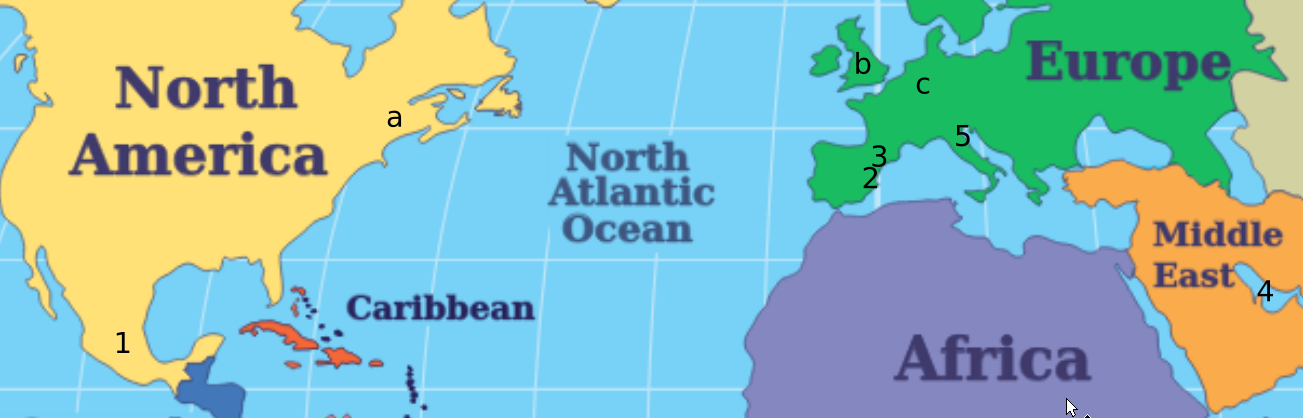
\includegraphics[width=120mm]{img/01_dit_compthink_map.png}
\end{center}

\begin{columns}
\footnotesize
\begin{column}{0.5\textwidth}

\begin{enumerate}
 \item BEng in Computing at UNAM, Mexico
%  \footnote{\url{https://www.unam.mx}}
 
	MSc in Computing at UNAM, Mexico
	\vspace{-1mm}
	
	\begin{itemize}
	 \item Internship at UdeM, Canada
	\end{itemize}						\pause 
	
 \item MSc in AI at UPV, Spain
 
 PhD in AI at UPV, Spain
 \vspace{-1mm}
 
 \begin{itemize}
	 \item Internship at UofS, UK%
% 	 \footnote{\url{https://www.sheffield.ac.uk}}
	\end{itemize}						\pause 
\end{enumerate}
\end{column}

\begin{column}{0.5\textwidth}

\begin{enumerate}\setcounter{enumi}{2}
 \item Post-doc at UPC, Spain
 \vspace{-1mm}
 
	\begin{itemize}
	 \item Internship at BUW, Germany
	\end{itemize}							\pause 

 \item Scientist at QCRI, Qatar				\pause 
 \bigskip 
 
 \item Professor at UniBO, Italy
\end{enumerate}
\vspace{1mm}
\end{column}
\end{columns}
\end{frame}

\begin{frame}
\frametitle{PhDs that I am supervising}

\alert{\textit{4th} year (about to graduate)}

\textbf{Arianna Muti} 

Hidden in Plain Sight: Detecting Misogyny beneath Ambiguities and Implicit Bias 
in Language				\pause 

\begin{itemize}
 \item Internship at Expert.ai (Modena, Italy)
 \item Internship at U. of Groningen (Groningen, The Netherlands)
 \item 10+ peer-reviewed full papers published (one upcoming at EMNLP)
 \item Transitioning towards a PostDoc at Bocconi University
\end{itemize}					\pause 


\textbf{Katerina Korre}

A Universal and Cross-language Approach to Internet Hate Speech Detection and
Analysis			\pause 

\begin{itemize}
 \item Internship at Symanto.ai (Valencia, Spain)
 \item 8+ peer-reviewed full papers published (two under review in journals)
 \item Transitioning towards a PostDoc at Athens University
\end{itemize}
\end{frame}

\begin{frame}
\frametitle{PhDs that I am supervising}

\alert{2nd year}

\textbf{Paolo Gajo}

NLP Technologies for Gastronomy			\pause

\begin{itemize}
 \item Internship at Dalhousie University (Halifax, Canada)
 \item 4+ peer-reviewed full papers published (two during his masters)
\end{itemize}						\pause 
\bigskip

\alert{Unfinished}

\textbf{Francesco Fernicola}

Return to the Source: Assessing Machine Translation Suitability	\pause 


\begin{itemize}
 \item In co-supervision with EURAC Research (Bolzano, Italy)
 \item 5+ peer-reviewed full papers published (two during his masters)
 \item Currently Computational Linguist at the European Parliament
\end{itemize}


\end{frame}


\begin{frame}
\frametitle{Computing at DIT}
\framesubtitle{Recent and ongoing research projects%
\footnote{Non exhaustive}} 

\begin{itemize}
 \item \alert{UpSkills} on upgrading the (technological) skills of language 
students
	\light{\url{https://upskillsproject.eu}}
\bigskip	\pause 

 \item \alert{UNITE} on exploiting LLMs for language learning
 	\light{\url{http://site.unibo.it/unite}}
\bigskip	\pause

 \item \alert{!Translate} on augmenting machine translation with explanations
 \light{\url{https://site.unibo.it/no-translate}}
\bigskip	\pause 
 
 \item \alert{Gastrowiki} on producing and fixing definitions
	\light{\url{https://site.unibo.it/gastrowiki}}
\end{itemize}
\end{frame}

\begin{frame}
\frametitle{Computing at DIT}
\framesubtitle{Computing Power%
\footnote{Dedicated to deep learning (training and out-of-the-box)}} 

\begin{itemize}
 \item 4 NVIDIA RTX 6000 Ada
\light{\footnotesize 
\url{https://www.nvidia.com/en-us/design-visualization/rtx-6000}}
\bigskip

\item 2  NVIDIA Quadro P4000

\light{\footnotesize
\url{https://www.techpowerup.com/gpu-specs/quadro-p4000.c2930}}
\end{itemize}
\vspace{5mm}

\centering
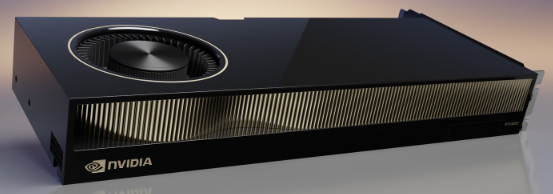
\includegraphics[width=65mm]{img/01_dit_compthink_nvidia.png}

\end{frame}

\begin{frame}
\frametitle{Lesson coordinates}
Slides and code available at:
\bigskip

\faFirefox\, \url{https://albarron.github.io/teaching/phd-comp-thinking/}

\end{frame}

\begin{frame}
\frametitle{Tools}

\alert{Python 3} programming language

We will use Google's Colab: \url{https://colab.research.google.com}
\bigskip 

For (more) serious affairs, you could consider
\begin{enumerate}
	\item Command line \alert{or}
	\item Integrated development environment; e.g.,
	Pycharm\footnote{\url{https://www.jetbrains.com/pycharm/}},
	Eclipse\footnote{\url{https://www.eclipse.org/}} \alert{or}
	local Jupyter%
\footnote{\url{https://jupyter.org/}}
\end{enumerate}
\end{frame}

\begin{frame}
\section{Contents}
\centering
\alert{Contents}
\end{frame}

\begin{frame}
 \frametitle{Lesson contents}
\alert{Introduction to computational thinking}

\begin{enumerate}
 \item Problem definition and solving
 \item Decomposition
 \item Pattern recognition
 \item Abstraction
 \item Algorithmic thinking
\end{enumerate}
\bigskip 	\pause 

\alert{Programming}
\begin{enumerate}\setcounter{enumi}{5}
 \item Introduction to programming
 \item Jupyter notebooks
 \item Basic operations
 \item Dealing with text
\end{enumerate}
\end{frame}


\begin{frame}
\section{Computational Thinking}
\centering
\alert{Computational Thinking}
\end{frame}





\begin{frame}
\frametitle{}
The tools we use have a profound and devious influence on our thinking habits, 
and therefore on our thinking abilities.
\begin{flushright}
Edsger W. Dijkstra%
\footnote{\url{https://amturing.acm.org/award_winners/dijkstra_1053701.cfm}}
\end{flushright}
\end{frame}

% \begin{frame}
% \frametitle{Table of Contents}
% \tableofcontents
% \end{frame}


\begin{frame}
\frametitle{Computational Thinking}
``[Computational Thinking] represents a universally applicable attitude and
skill set \alert{everyone}, not just computer scientists, would be eager to
learn and use''
\begin{flushright}
	Jeannette M. Wing, CMU (\citeyear{Wing2006})
\end{flushright}
\end{frame}


\begin{frame}
\frametitle{Humans and Computers}

Computational methods and models give us the \textit{courage} to solve problems 
and design systems
\bigskip 			\pause

Computational thinking confronts the riddle of machine intelligence:
\begin{itemize}
 \item What can humans do better than computers?

\item What can computers do better than humans?
\bigskip											\pause

\alert{Some examples of each?}
\bigskip 											\pause

\item What is computable?
\end{itemize}
\end{frame}

\begin{frame}
\frametitle{A few definitions}
\begin{columns}
\begin{column}{0.2\textwidth}
 
\includegraphics[width=23mm]{img/homer_marketing.png}
\end{column}												\pause

\begin{column}{0.8\textwidth}

\alert{Problem}
\begin{enumerate}
 \item A difficulty that has to be resolved or dealt with
 \item A question to be answered, schoolwork exercise	\pause

	\textbf{Antonyms}: solution
\end{enumerate}											\pause

\alert{System}
\begin{enumerate}
 \item A group of interacting or interrelated elements that act according to a
set of rules to form a unified whole
\end{enumerate}											\pause

\alert{Computability}
\begin{enumerate}
 \item The ability to solve a problem in an effective manner
\end{enumerate}

\end{column}
\end{columns}
\bigskip

\onslide
\footnotesize
\light{%
\url{https://en.wiktionary.org/wiki/problem}	\\
\url{https://en.wikipedia.org/wiki/System}	\\
\url{https://en.wikipedia.org/wiki/Computability}
}
\end{frame}

\begin{frame}
\frametitle{Activity 1: The Seven Bridges of K\"onigsberg}

\alert{Task}: Devise a path through the city of K\"onigsberg that would cross
each of the bridges once and only once

\begin{center}
 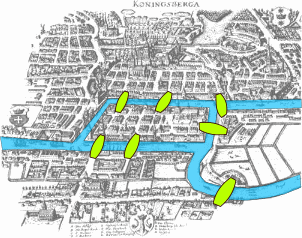
\includegraphics[width=80mm]{img/Konigsberg_bridges.png}
\end{center}
\end{frame}

\begin{frame}
 \frametitle{Activity 1: The Seven Bridges of K\"onigsberg}
\framesubtitle{Looking for a solution}							\pause

\begin{center}
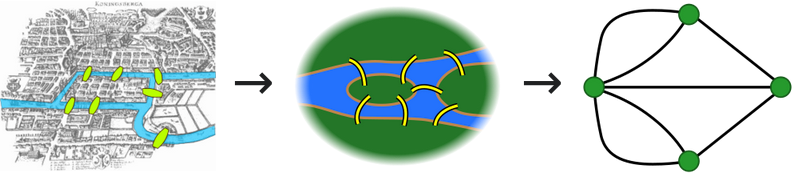
\includegraphics[width=120mm]{img/Konigsberg_bridges_graph.png}
\end{center}
\bigskip 								\pause

Can you devise a solution using this \alert{abstraction}?
\bigskip 								\pause

\alert{Solution}: There is no solution 				\pause


\begin{columns}
\begin{column}{0.45\textwidth}

The foundations of graph theory

Leonhard Euler (1736)
\end{column}
\begin{column}{0.4\textwidth}

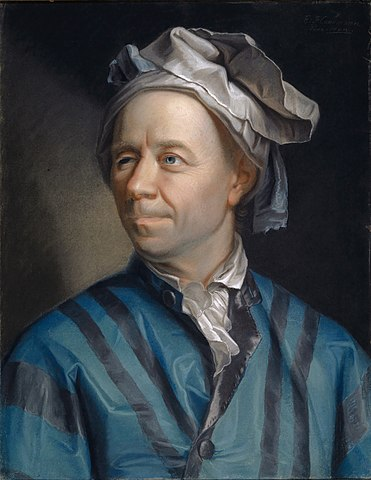
\includegraphics[width=16mm]{img/371px-Leonhard_Euler.jpeg}
\end{column}
\end{columns}
\end{frame}


\begin{frame}
\frametitle{What is involved in computational thinking}

\begin{itemize}
 \item Defining problems				\pause 
 \item Solving problems					\pause
 \item Designing systems				\pause
 \item Understanding human behavior
\end{itemize}
\bigskip

All by drawing on the concepts fundamental to computer science
\bigskip 									\pause

\begin{itemize}
 \item How difficult is it to solve?			\pause
 \item What’s the best [doable$\mid$acceptable$\mid$affordable] way to solve it?	
\pause
 \item An approximate solution is good enough?	\pause
 \item False positives or false negatives are allowed?	\pause
\end{itemize}
\begin{center}
\begin{tabular}{cccc}
                 &              & \multicolumn{2}{c}{\alert{predicted label}}   
\\
                 &              &  positive     & negative      \\\cline{3-4}
\alert{true}& \multicolumn{1}{l|}{positive}& true positive      & 
\multicolumn{1}{l|}{false positive}\\
\alert{label}& \multicolumn{1}{l|}{negative}& false negative& 
\multicolumn{1}{l|}{true negative} \\\cline{3-4}
\end{tabular}
\end{center}
\end{frame}

\begin{frame}
\frametitle{How to deal with a difficult problem?}

[By] reformulating a seemingly difficult problem into one we know how to solve, 
perhaps by reduction, embedding, transformation, or simulation	\pause
\medskip

[\ldots] using abstraction and decomposition when attacking a large complex task 
or designing a large complex system
\bigskip 		\pause

Have \alert{you} solved a problem using any of these techniques?	\pause
\bigskip					\pause

\alert{Copying a drawing?}

\light{\url{https://www.wikihow.com/Copy-a-Drawing-or-Picture-by-Hand}}
\end{frame}

\begin{frame}
\frametitle{The thinking in computational thinking}

Thinking in terms of \ldots
\begin{itemize}
 \item Prevention		\pause

 Do \alert{you} backup your mobile phone?		\pause

 There are two kinds of people
 \begin{enumerate}
  \item those who backup
  \item those who have never lost all their data [mobile phone]
 \end{enumerate}							\pause

 \item Protection				\pause

 Do \alert{you} use a case to protect your mobile phone?	\pause
\end{itemize}
\bigskip

Getting ready to recover from worst-case scenarios through
\medskip

\centering
\begin{tabular}{l@{\hspace{1mm}}c@{\hspace{1mm}}p{0.5\textwidth}}
redundancy	& $\rightarrow$	&
If I keep money in my backpack, I can go home even if I loose my wallet \\\pause

damage containment	& $\rightarrow$	&
If I have an exam, I will take an earlier train than usual	\\		\pause

error correction	& $\rightarrow$	&
Before handling my report, I will pass a spell checker	\\
\end{tabular}
\end{frame}


\begin{frame}
\frametitle{Computational thinking is search, search, and more search}
\pause

How do \alert{you}
\begin{itemize}
 \item Buy the best possible item on Amazon?
 \item Find the best match on Tinder?
 \item Spot the most entertaining tiktok?
\end{itemize}						\pause
\bigskip

\begin{columns}
\begin{column}{0.45\textwidth}
How do \alert{you} win at UNO?		\pause
\bigskip

How do \alert{you} win at dominoes?		\pause
\bigskip

How do \alert{you} win at chess?

\centering
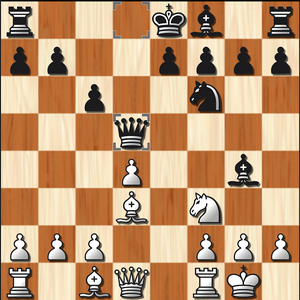
\includegraphics[width=30mm]{img/chess.png}
\end{column}							\pause

\begin{column}{0.5\textwidth}
How do \textit{standard \alert{computers}} win at chess?
\bigskip								\pause

\centering
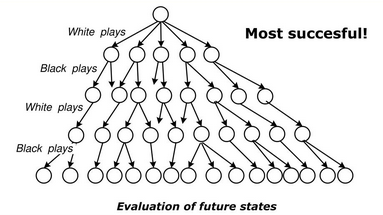
\includegraphics[width=60mm]{img/chess_brute.png}
\bigskip
\end{column}
\end{columns}
\end{frame}

%  FROM LESSON 3
\begin{frame}
\frametitle{What computational thinking is and is not}
\framesubtitle{Characteristics}

\alert{Conceptualising, not programming}

\begin{itemize}
 \item Computer science is \alert{not} computer programming
 \item Beyond ($\sim$beside) being able to program a computer
 \item Thinking at multiple levels of abstraction
\end{itemize}			\pause

\alert{Fundamental skill}
\begin{itemize}
 \item A skill every human being must know to function in modern society
\end{itemize}	\pause

\alert{A way that humans, not computers, think}
\begin{itemize}
 \item A way humans solve problems
 \item Not trying to get humans to think like computers
\end{itemize}							\pause

\centering
\begin{tabular}{l}
Computers are dull and boring		\\	\pause 
Humans are clever and imaginative	\\	\pause  
Humans make computers exciting		\\	\pause 
\end{tabular}
\end{frame}

\begin{frame}
\frametitle{Computational Thinking: The three As}

An iterative process based on three stages:

\begin{description}
	\item[\textbf{A}bstraction]	(Problem Formulation).
		One attempts to conceptualize a problem verbally, e.g., by trying to 
formulate a question such as ``How does gravity work?,'' or through visual 
thinking, e.g., by drawing a diagram identifying objects and relationships
		\pause

	\item[\textbf{A}utomation]	(Solution Expression).
	 	It is expressed in a non-ambiguous way so that the computer	can carry 
it 
out; e.g., through computer programming \light{(or through \textit{prompting}?)}
		\pause

	\item[\textbf{A}nalysis]  (Execution \& Evaluation).
	The solution gets executed (by the computer) in ways that show the direct 
consequences of one's own thinking. Visualisations could support the evaluation 
of solutions
\end{description}

\onslide
\flushright
\footnotesize
\citep{Repenning:16}
\end{frame}

% From lesson 4

\begin{frame}
\frametitle{Algorithm}

An algorithm is\ldots 
\bigskip

\begin{description}
 \item[Definition 1]
A finite sequence of \alert{well-defined (computer-implementable) 
instructions}, typically to solve a class of problems or to perform a 
computation

\begin{flushright}
\url{https://en.wikipedia.org/wiki/Algorithm}
\end{flushright}
\bigskip 			\pause 

\item[Definition 2]
An explicit, precise, unambiguous, mechanically-executable sequence of 
elementary instructions, usually intended to accomplish a specific purpose. 

\begin{flushright}
\citet[p. 1]{Erickson:19} 
\end{flushright}
\end{description}

\end{frame}

\begin{frame}
\frametitle{Activity 2: The panino%
\footnote{Since recipes are \textit{just} algorithms}
}

\alert{Problem:} Write the algorithm to prepare a \textit{panino}
\end{frame}

\begin{frame}
\frametitle{Activity 6: The panino}

\alert{My} algorithm to prepare a \textit{panino}%
\footnote{Via Taranto from \url{https://ilpaninobologna.com}}	\pause 

\textbf{Ingredients}: 

bread $\bullet$ \textit{prosciutto crudo $\bullet$ pecorino di Pienza $\bullet$ 
carciofini sott'olio}	\pause 
\begin{enumerate}
 \item Cut the bread into two halves horizontally		\pause 
 \item Add three slices of \textit{prosciutto} on top of the bottom half	
 
	* get sure not to go beyond the border of the bread			\pause 
 \item Evenly distribute some slices of \textit{pecorino}		\pause
 \item Add 3 pieces of \textit{carciofini}
 
		* get sure not to get too much oil\pause
 \item Put the top half of bread on top					\pause
 \item Enjoy
\end{enumerate}
\end{frame}

\begin{frame}
\frametitle{Activity 6: The panino}

Possible \textit{issues} in \alert{your/my} recipes%
\footnote{Keep in mind that this is a toy problem}
\bigskip 

\begin{itemize}
 \item Under-specification?						\bigskip	\pause 
 \item Lack of identification of the input?		\bigskip	\pause 
 \item Imprecise identification of the problem?
\end{itemize}
\end{frame}

\begin{frame}
\frametitle{Describing Algorithms}

The 4 components of an algorithm

\begin{description}
 \item[What:] A precise specification of the problem that the algorithm solves
	\pause 
 \item[How:] A precise description of the algorithm itself			\pause 
 \item[Why:] A proof that the algorithm solves the problem it is supposed to 
solve%
\footnote{Not covered in this lesson}			\pause 
 \item[How fast:] An analysis of the running time of the algorithm%
\footnote{idem}
\end{description}	\pause 

\begin{itemize}
 \item No particular development order				\pause 
 \item Write for an audience; this is not intended for yourself \pause 
 \item Write for people who is not as clever as you are%
\footnote{For instance, yourself 6 months ago}
\end{itemize}

\onslide 
From~\cite[p. 11]{Erickson:19}
\end{frame}

% From lesson 5
\begin{frame}
\frametitle{Natural vs Programming languages}

\alert{Natural languages}

\begin{itemize}
\item An \textit{ordinary} language (e.g., Italian)
\item Written or oral
\item It has evolved naturally in humans, usually without specific and 
deliberate planning%
\footnote{Consider Klingon or Sith}
\item \textit{Problem}: ambiguity

(e.g., ``visiting relatives can be annoying'')
\end{itemize}
\pause

\alert{Programming languages}
\begin{itemize}
\item Formal-born languages
\item Specific syntactic rules that avoid ambiguous statements
\item \textit{Sentences} convey one single meaning
\item They can have a significant degree of abstraction
\end{itemize}
\end{frame}

\begin{frame}
\frametitle{Programming language}

A formal language comprising a set of instructions that produce various kinds 
of 
output [given an input]%
\footnote{\url{https://en.wikipedia.org/wiki/Programming_language}}
\bigskip
\pause

\begin{center}
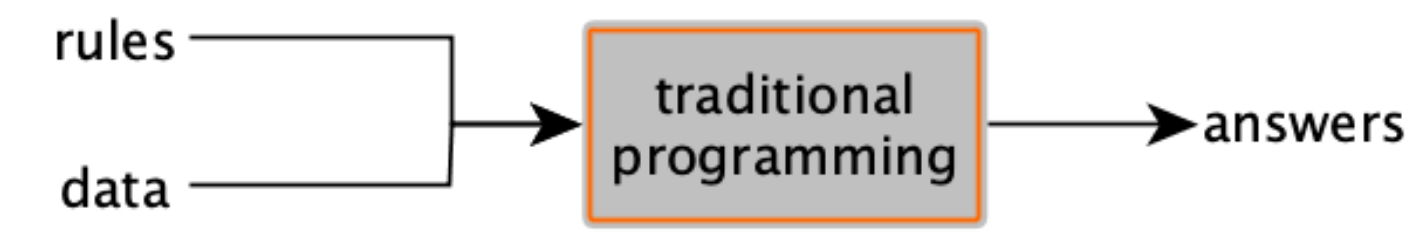
\includegraphics[width=83mm]{img/01_programming.png}
\end{center}
\bigskip 

\footnotesize \light{Diagram from L. Moroney's Introduction to TensorFlow for 
Artificial Intelligence, Machine Learning, and Deep Learning}
\end{frame}



\begin{frame}[allowframebreaks]
\frametitle{References}
\bibliographystyle{humannat}
\bibliography{compthink}
\end{frame}

\end{document}
